% \documentclass{standalone}
% \usepackage{tikz}
% \usepackage{amsmath}

% \begin{document}
% \begin{tikzpicture}[scale=1]

%   % Axes
%   \draw[->] (-2.5,0) -- (2.5,0) node[right] {$x$};
%   \draw[->] (0,-2.5) -- (0,2.5) node[above] {$y$};

%   % Define the radius of the circle
%   \def\r{2}

%   % Circle
%   \draw[red] (0,0) circle (\r);

%   % Square (coordinates calculated based on the radius)
%   \draw[blue!80, thick] (\r,0) -- (0,\r) -- (-\r,0) -- (0,-\r) -- cycle;

%   % Points and labels
%   \draw[fill=blue!80] (cos(23*\pi/16),sin(23*\pi/16)) circle (1pt) node[below right] {$k=3$};
%   \draw[fill=blue!80] (0,\r) circle (1pt) node[above right] {$k=0$};
%   \draw[fill=blue!80] (-\r,0) circle (1pt) node[above left] {$k=1$};
%   \draw[fill=blue!80] (0,-\r) circle (1pt) node[below left] {$k=2$};

% \end{tikzpicture}
% \end{document}

\documentclass{standalone}
\usepackage{tikz}
\usepackage{amsmath}

\begin{document}
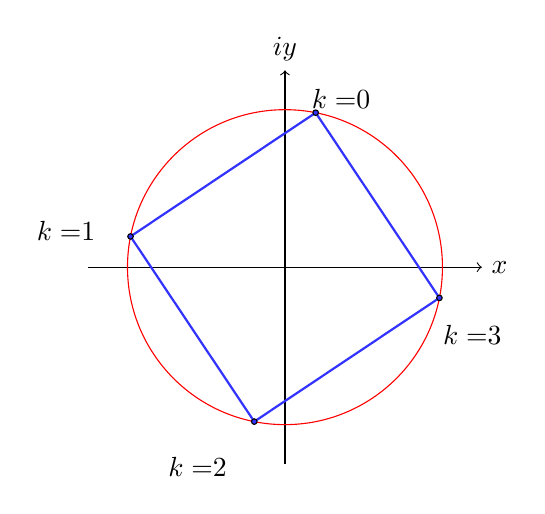
\begin{tikzpicture}[scale=1]

  % Axes
  \draw[->] (-2.5,0) -- (2.5,0) node[right] {$x$};
  \draw[->] (0,-2.5) -- (0,2.5) node[above] {$iy$};

  % Define the radius of the circle
  \def\r{2}

  % Circle
  \draw[red] (0,0) circle (\r);

  % Square (coordinates calculated using polar coordinates)
  \draw[blue!80, thick]
    ({cos((7*pi/4 + 2*pi*0)/4 r)*\r}, {sin((7*pi/4 + 2*pi*0)/4 r)*\r}) --
    ({cos((7*pi/4 + 2*pi*1)/4 r)*\r}, {sin((7*pi/4 + 2*pi*1)/4 r)*\r}) --
    ({cos((7*pi/4 + 2*pi*2)/4 r)*\r}, {sin((7*pi/4 + 2*pi*2)/4 r)*\r}) --
    ({cos((7*pi/4 + 2*pi*3)/4 r)*\r}, {sin((7*pi/4 + 2*pi*3)/4 r)*\r}) --
    cycle;

%   \draw[blue!80, thick] ({cos((7*pi/4 + 2*pi*0)/4 r)*\r}, {sin((7*pi/4 + 2*pi*0)/4 r)*\r}) -- (0,\r) -- (-\r,0) -- (0,-\r) -- cycle;


    % \draw[blue!80, thick] 
    % ({cos((7*pi/4 + 2*pi*0)/4)*\r}, {sin((7*pi/4 + 2*pi*0)/4)*\r}) --
    % ({cos((7*pi/4 + 2*pi*1)/4)*\r}, {sin((7*pi/4 + 2*pi*1)/4)*\r}) --
    % ({cos((7*pi/4 + 2*pi*2)/4)*\r}, {sin((7*pi/4 + 2*pi*2)/4)*\r}) --
    % ({cos((7*pi/4 + 2*pi*3)/4)*\r}, {sin((7*pi/4 + 2*pi*3)/4)*\r}) -- cycle;

    % \draw[blue!80, thick]
    % foreach \k in {0,1,2,3} {
    % ({cos((7*pi/4 + 2*pi*\k)/4)*\r}, {sin((7*pi/4 + 2*pi*\k)/4)*\r}) --
    % } cycle;


  % Points and labels (using a loop for efficiency)
  \foreach \k in {0,1,2,3} {

  %   \draw[fill=blue!80] (0,\r) circle (1pt) node[above right] {$k=0$};
    \pgfmathsetmacro{\angle}{(7*pi/4 + 2*pi*\k)/4}
    \pgfmathsetmacro{\x}{\r*cos(\angle r)} % 'r' for radians
    \pgfmathsetmacro{\y}{\r*sin(\angle r)} % 'r' for radians
    \draw[fill=blue!80] (\x,\y) circle (1pt) node[label={[shift={(-0.2,-0.2)}]\angle*180/pi:$k=$\k}] {};
  }

\end{tikzpicture}
\end{document}